\section{Discussion}

Let we demonstrate our algorithm in example. Reference language is specified with grammar $G$:\\
(0) start\_rule ::= s \\
(1) s ::= LBR s RBR s\\
(2) s ::= $\varepsilon$ \\

We suppose that regular approximatoin calculation and its tokenization performed, 

\begin{figure}
    \begin{center}
        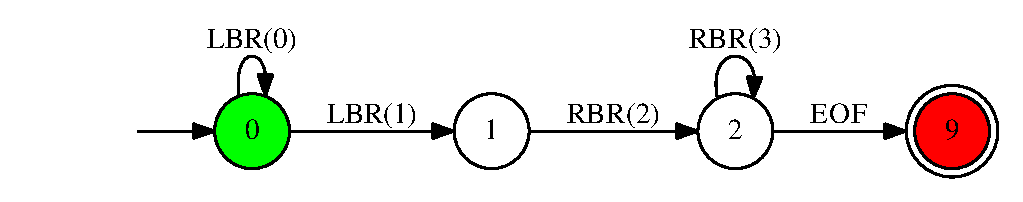
\includegraphics[scale=0.5]{dot/in3.eps}
    \end{center}
    \caption{Input for our algorithm: regular approximation for some code after tokenization} 
    \label{faApprox}
\end{figure}

\begin{figure}
    \begin{center}
        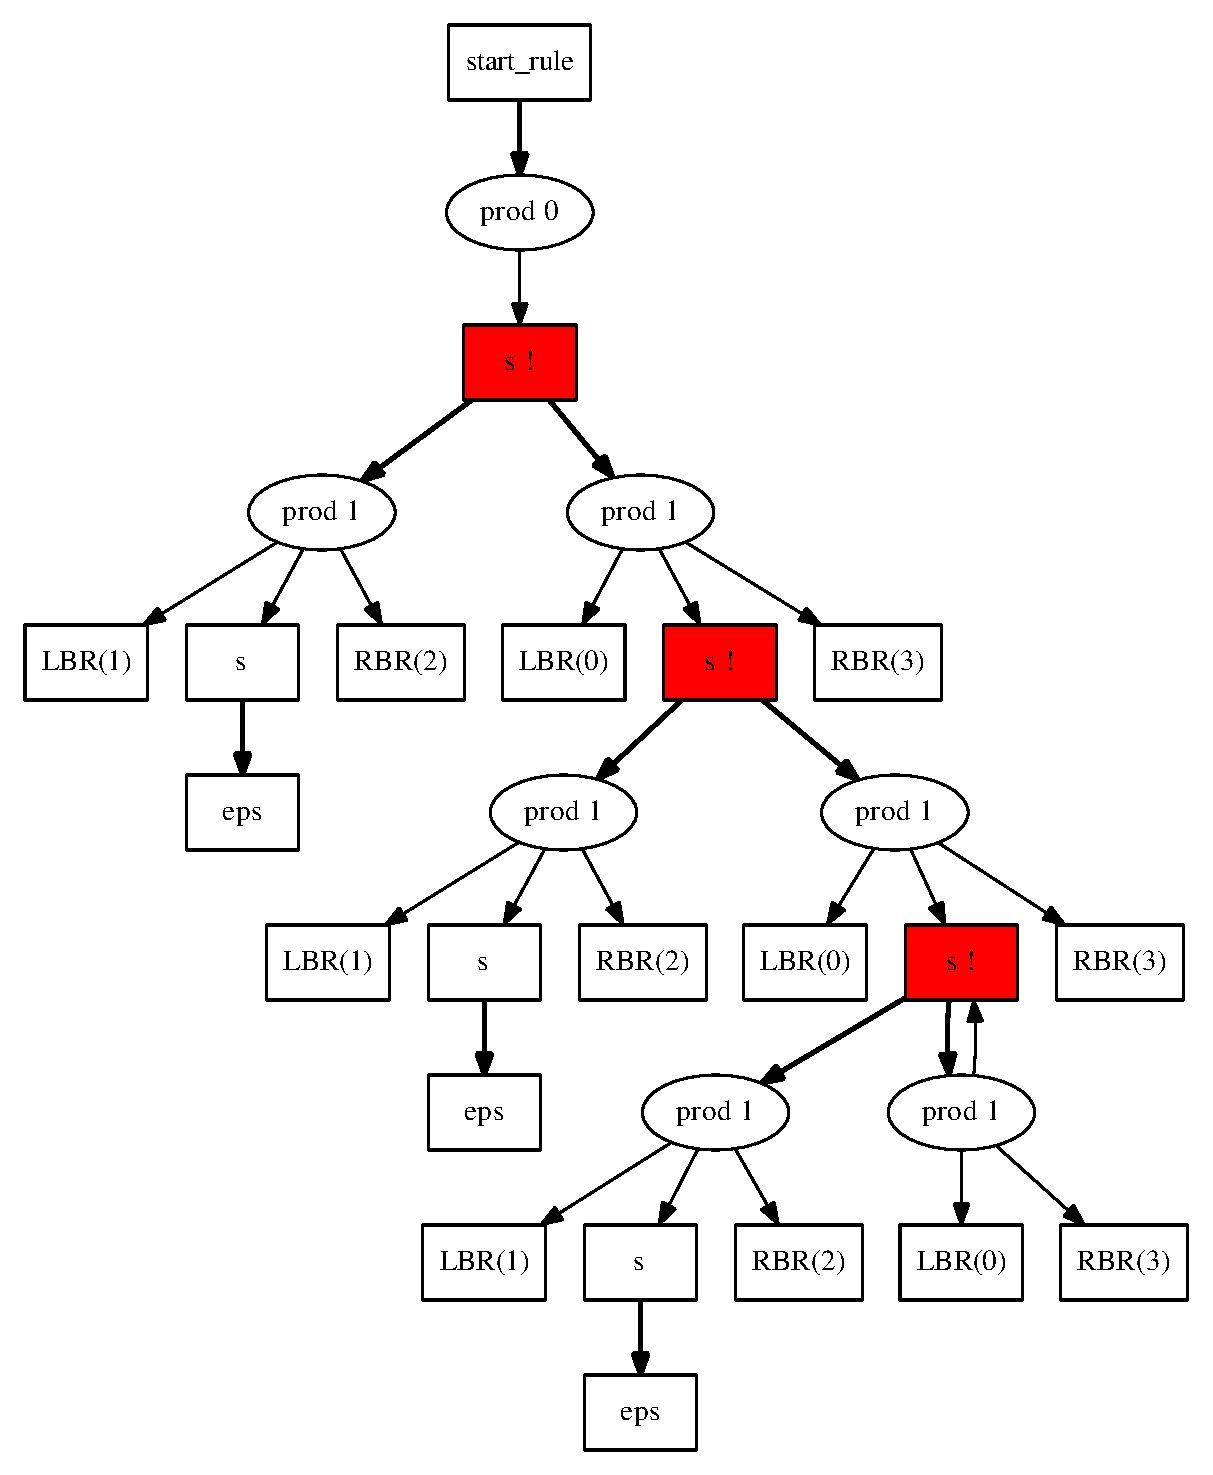
\includegraphics[scale=0.5]{dot/out3.eps}
    \end{center}
    \caption{SPPF for input presented in figure~\ref{faApprox}}
    \label{resultSPPF}
\end{figure}



Presented algorifm notify about errors in input automata only if $L_a \cap L_r = \emptyset$. There are two possible ways to solve this problem.
We can previously check correctness and report all errors and then apply our algorithm for forect construction of correct subset.
The other way is modification of our algorithm such way that for input regular set it returns forest for all correct sentences in $L_a$ 
and notify about incorrect sentences if they exist.

Full theoretical estimation of string-embedded languages parsing complexity in depends on input is not provided 
in known works, so it is open question for future reserach.

Described algorithm produce SPPF which utilizes for trees extraction and sematic calculation in original RNGLR. Semantic actions may be smecified by using attributed grammar.
Semantic procssing and transformations for string-embedded languages may be useful, for examplr, for migration to more principal aproaches of dynamic code generattion, as proposrd in~\cite{EvalToStaged}.
We also can use this approac to specify semantic, but unfortunately in our case SPPF contains cycles which cannot be elaminated, so termination 
and correctness of semantic calcualtion and transformation is topic for research. 

% Context-free approximation processing?
% Implementation in IDE?  
